\newlength\psSpinBallRadius
\setlength{\psSpinBallRadius}{0.8\unitlength}

\def \psSpinUpBall {\pst@object{psSpinUpBall}}
\def \psSpinUpBall(#1){{%
   \rput(#1){%
      \psline[linecolor=black, linewidth=0.2\psSpinBallRadius, arrowscale=2]{->}(0,-2\psSpinBallRadius)(0,2.5\psSpinBallRadius)
      \psBall{gray}{\psSpinBallRadius}
      \psellipticarc[linecolor=black, linewidth=0.1\psSpinBallRadius, arrowscale=1.5, fillstyle=none]{->}(0,-1.7\psSpinBallRadius)(1.0\psSpinBallRadius,0.35\psSpinBallRadius){-60}{250}%
   }
}}

\def \psSpinDownBall {\pst@object{psSpinDownBall}}
\def \psSpinDownBall(#1){{%
   \rput(#1){%
      \psline[linecolor=black, linewidth=0.2\psSpinBallRadius, arrowscale=2]{<-}(0,-2.5\psSpinBallRadius)(0,2\psSpinBallRadius)
      \psBall{gray}{\psSpinBallRadius}
      \psellipticarc[linecolor=black, linewidth=0.1\psSpinBallRadius, arrowscale=1.5, fillstyle=none]{<-}(0,1.7\psSpinBallRadius)(1.0\psSpinBallRadius,0.35\psSpinBallRadius){-70}{240}%
   }
}}



\newcommand{\posterPolarization}[1]{

\setlength{\frameWidth}{#1}
\setlength{\unitlength}{0.02\frameWidth}
\psset{unit=\unitlength}

\rput[t](43,30){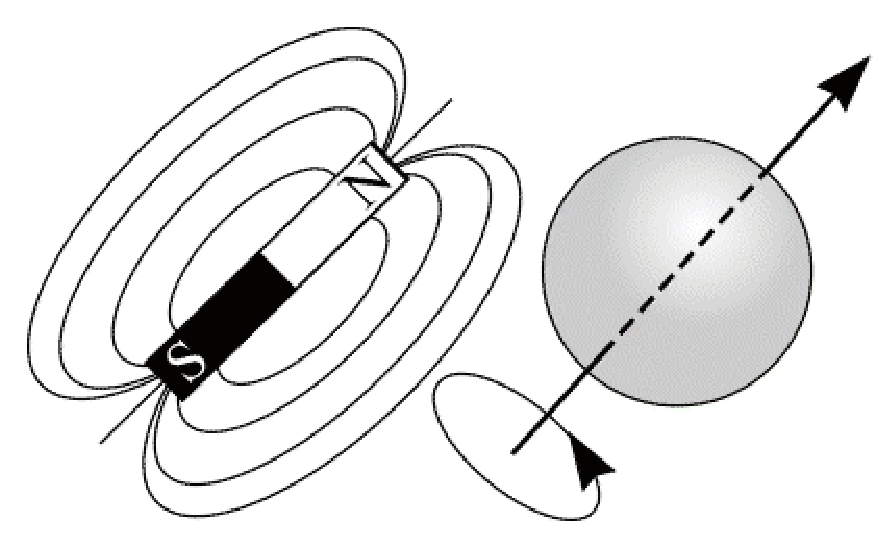
\includegraphics[width=12\unitlength]{graphics/mmom3}}
\rput[t](47,30){\Large $\vec\mu$}

\rput[lt](2,30.3) {%
\begin{minipage}{47\unitlength}

\raggedright

\begin{list}{\labelitemi}{\setlength{\itemsep}{-0.5\unitlength}
                          \setlength{\topsep}{0mm}
                          \setlength{\leftmargin}{0mm}
                          \setlength{\rightmargin}{0mm}}

   \item Electrically charged particles possess a magnetic moment
   \Large%
   \begin{equation*}
   \hspace{-60mm}
   \vec\mu \propto\frac{q}{m} \vec{s}
   \end{equation*}

   \small
   \begin{list}{\labelitemii}{\setlength{\itemsep}{2mm}}
      \item In classical mechanics particle simply spins around its center of mass
      \item In quantum mechanics \textbf{spin is a truly intrinsic property of particle}% (like mass and charge)
   \end{list}

   \normalsize
   \item Spin can have only two orientations in space: ``up'' and ``down'' along $Z$

   \item Polarization $P$ is a fraction of particles contributing to total momentum

\end{list}

\end{minipage}
}

\rput(25,10){ \psframebox{\Large $ P =  \frac{N_\uparrow - N_\downarrow}{N_\uparrow + N_\downarrow}$ } }

\psline[linewidth=0.2, arrowscale=2]{->}(2,0)(2,7)
\rput(1,7){\large $Z$}

\rput[t](9,0.5){\large $P = 100\%$}

\psSpinUpBall(5,4)
\psSpinUpBall(7,5)
\psSpinUpBall(8.5,3.5)
\psSpinUpBall(10.5,4.3)
\psSpinUpBall(13,4.9)
\psSpinUpBall(12,3)

\rput[t](24,0.5){\large $P = 0\%$}

\psSpinUpBall(20,4)
\psSpinDownBall(22,5)
\psSpinUpBall(23.5,3.5)
\psSpinDownBall(25.5,4.3)
\psSpinUpBall(28,4.9)
\psSpinDownBall(27,3)

\rput[t](40,0.5){\large $P \approx 67\%$}

\psSpinUpBall(35,4)
\psSpinUpBall(37,5)
\psSpinUpBall(38.5,3.5)
\psSpinUpBall(40.5,4.3)
\psSpinUpBall(43,4.9)
\psSpinDownBall(42,3)

%\rput{0}{\psgrid[gridlabels=0.7,subgriddiv=0, griddots=3](1,-1)(0,0)(\myPsPictureWidthLocal,\myPsPictureHeightLocal)}

}

\setlength{\unitlength}{10mm}
\psset{unit=\unitlength}
